\title{Lecture 4\\External Information Representation Languages}

\begin{frame}
	\titlepage
\end{frame}

\begin{frame}{\\Lecture Contents}
	\topline
	\justifying
	The graphical language for the external representation of SC-code constructs --- SCg-code. The syntax and denotational semantics of the SCg-code. The linear language for the external representation of SC-code constructs --- SCs-code. The syntax and denotational semantics of the SCs-code. The structured hypertext language for the external representation of SC-code constructs --- SCn-code.
\end{frame}

\begin{frame}{\\The concept of external languages}
	\topline
	\justifying
	\begin{SCn}
		\scnheader{external language}
		\scnidtf{language for representing information that human can see and understand}
		\scnidtf{messaging language}
		\begin{scnrelfromset}{examples}
			\scnitem{SCn-code}
			\scnitem{SCs-code}
			\scnitem{SCg-code}
		\end{scnrelfromset}
		
		\scnheader{internal language}
		\scnidtf{language for representing information in the memory of a cybernetic system}
	\end{SCn}
	
\end{frame}

\begin{frame}
	\centering
	\Huge
	SCg-code
\end{frame}

\begin{frame}{\\SCg-code}
	\topline
	\justifying
	\vspace*{\fill}
	\footnotesize
	\begin{SCn}
		\scnheader{SCg-code}
		\scnidtf{Semantic Code graphical}
		\scnidtf{Language for visual (graphical) representation of knowledge bases of ostis-systems}
		\scniselement{graph language}
		\scntext{explanation}{\textit{SCg-code} is a way of visualizing \textit{sc-texts} (information constructs of the SC-code) in the form of drawings of these abstract constructs.\\
			
		Let us emphasize that an abstract \textit{graph structure} and its drawing (graphic image) are not the same thing, even if they are isomorphic to each other.}
		
		\scntext{explanation}{\textit{SCg-code} is considered by us as a union of the \textit{SCg-code core}, which provides an isomorphic graphic representation of any \textit{sc-text}, as well as several directions for expanding this core, ensuring increased compactness and "readability"{} of \textit{SCg-code texts (sc.g-texts).}}
	\end{SCn}
\end{frame}

\begin{frame}{\\SCg-code}
	\topline
	\justifying
	\vspace*{\fill}\\
	The main goal of the \textit{SCg-code} is to have clear syntactic graphic features of the images of \textit{sc.g-elements}, allowing one to easily identify and distinguish such classes of \textit{sc.g-elements} as:
	\begin{textitemize}
		\item \textit{sc.g-constants} (signs of constant entities) and \textit{sc.g-variables} (images of variables whose values are the corresponding sc-elements);
		\item \textit{sc.g-variables} whose values are {sc-constants}, and \textit{sc.g-variables} whose values are \textit{sc-variables};
		\item signs of permanent (stable) entities and signs of temporary (unstable, temporarily existing, situational) entities;
	\end{textitemize}
	
\end{frame}

\begin{frame}{\\SCg-code}
	\topline
	\justifying
	\begin{textitemize}
		\item \textit{sc.g-connectors} (binary link signs) and \textit{sc.g-elements} that are not \textit{sc.g-connectors};
		\item undirected \textit{sc.g-connectors (sc.g-edges)} and directed \textit{(sc.g-arcs)};
		\item \textit{sc.g-arcs of belonging} and \textit{sc.g-arcs} that are not such;
		\item \textit{sc.g-arcs of positive membership}, negative membership and fuzzy membership.
	\end{textitemize}
\end{frame}

\begin{frame}{\\SCg-code syntax}
	\topline
	\justifying
	\begin{SCn}
		\scnheader{SCg Core Code Alphabet}
		\scnidtf{Alphabet of sc.g-elements graphically depicting sc-elements}
	\end{SCn}
	% 	The table \textbf{"SCg-text. SCg-code alphabet"} contains a list of elements of the \textbf{SCg-code alphabet}. This list is formatted as \textit{sc.g-text} and represents an image of examples of all entered types of \textit{sc.g-elements} (one example of each type). Moreover, the specified examples of \textit{sc.g-elements} are divided into five groups.
\end{frame}

\begin{frame}{\\SCg-code syntax}
	\topline
	\justifying
	\vspace*{\fill}
	\begin{figure}[H]
		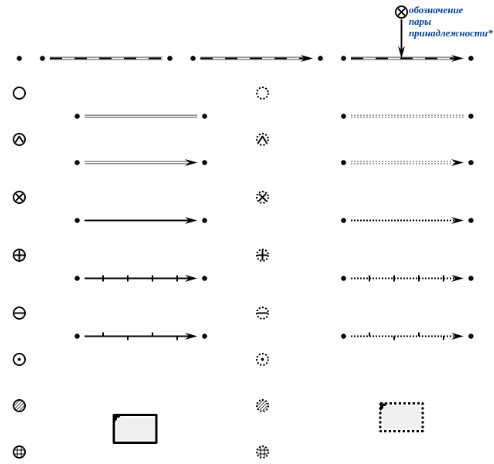
\includegraphics[scale=0.55]{./figures/external_langs/alphabet_scg_code_part1.png}
	\end{figure}
\end{frame}

\begin{frame}{\\SCg-code syntax}
	\topline
	\justifying
	\vspace*{\fill}
	\begin{figure}[H]
		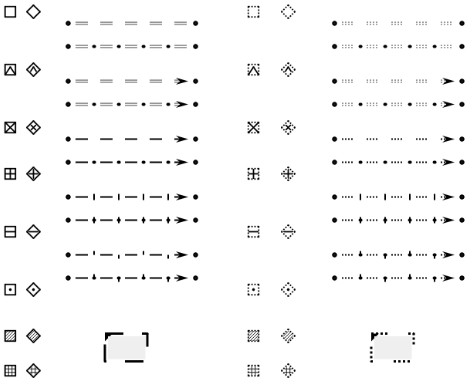
\includegraphics[scale=0.6]{./figures/external_langs/alphabet_scg_code_part2.png}
	\end{figure}
\end{frame}

\begin{frame}{\\SCg-code syntax}
	\topline
	\justifying
	\vspace*{\fill}\\
	The first group (top row) includes sc.g-elements, for which the constancy and permanence of the entities they denote require further clarification. The remaining four groups of sc.g-elements are similar to each other and include, respectively:
	\begin{textitemize}
		\item signs of \textbf{constant constant entities};
		\item signs of \textbf{constant temporary entities};
		\item images of \textit{sc-variables}, the values of which or the values of the values of which (if the values of the variables are variables) are the signs of constant constant entities;
		\item images of \textit{sc-variables} whose values or values of whose values (if the values of the variables are variables) are signs of constant temporary entities.
\end{textitemize}
\end{frame}

\begin{frame}{\\SCg-code syntax}
\topline
\justifying
A special place in the SCg-code is occupied by the representation of \textit{sc-elements}, which are \textit{designations of membership pairs*}, by explicitly using this \textit{\underline{semantically} distinguished class of sc-elements}. This \textit{sc.g-element} is used when we need to represent a \textit{sc-arc}, which is known to be a designation of a \textit{membership pair*}, but it is unknown what kind of membership we are talking about - a constant or a variable, or
permanent or temporary, positive, negative or unclear.
\end{frame}

\begin{frame}{\\SCg-code syntax}
\topline
\justifying
\vspace*{\fill}\\
In addition to the \textit{sc.g-elements} listed in the \textbf{“SCg-text. SCg-code alphabet”} table, the \textit{SCg-code alphabet} also includes the following \textit{sc.g-elements}:
\begin{textitemize}
	\item external identifiers of \textit{sc-elements}, identical to (assigned to) the corresponding \textit{sc.g-elements};
	\item \textit{sc.g-contour}, each of which is a sign of some \textit{sc-text} (a structure consisting of sc-elements);
	\item \textit{sc.g-frames} of increased size are the image limiters of various files stored in the memory of the ostis-system;
	\item \textit{sc.g-buses}, which are designations of the same entities as the \textit{sc.g-elements} incident to them.
\end{textitemize}
\end{frame}

\begin{frame}{\\SCg-code syntax}
\topline
\justifying
\vspace*{\fill}\\
We also note that, in addition to all the listed elements of the \textit{SCg-code Alphabet}, each of which has a well-defined denotational semantics, to formalize the syntax of the SCg-code it is necessary to introduce a whole series of "smaller"{}syntactic objects, for example:
\begin{textitemize}
	\item incidence points of \textit{sc.g-connectors} with \textit{sc.g-nodes}, with other \textit{sc.g-connectors, with sc.g-contours, with sc.g-frames};
	\item incidence points \textit{sc.g-tires};
	\item breakpoints of linear \textit{sc.g-elements (sc.g-connectors, sc.g-contours, sc.g-frames, sc.g-buses)}.
\end{textitemize}
\end{frame}
\iffalse
\begin{frame}{\\Denotational semantics of the SCg-code}
\topline
\justifying
\vspace*{\fill}\\
The SCg-code is divided into the \textit{SCg-code core} and its extensions. The \textit{SCg-code core alphabet} is the alphabet of \textit{sc.g elements}, graphically represented by \textit{sc elements}. The \textit{SCg-code core alphabet} corresponds one-to-one to the \textit{SC-code alphabet}.
The denotational semantics of the \textit{SCg-code core} corresponds to the denotational semantics of the SC-code.
\begin{figure}[H]
	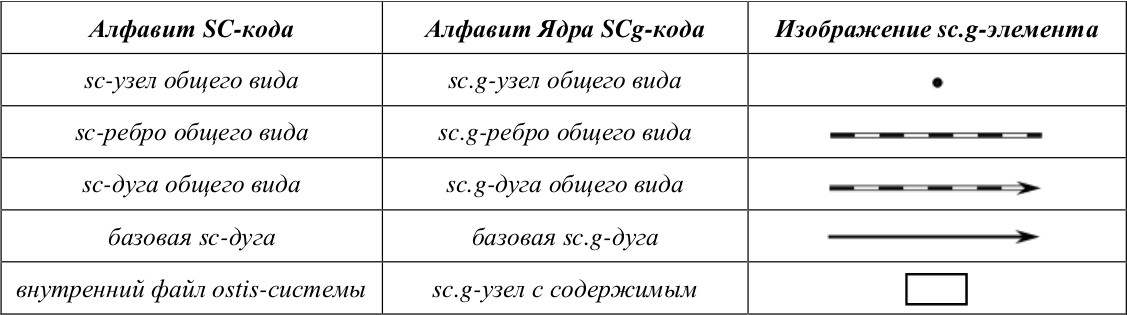
\includegraphics[scale=0.4]{./figures/external_langs/table_scg_code.png}
\end{figure}
\end{frame}

\begin{frame}{\\Denotational semantics of the SCg-code}
\topline
\justifying
\begin{SCn}
	\scnheader{\textit{sc-node} with content}
	\scnidtf{\textit{sc-node}, having content}
	\scnidtf{\textit{sc-node}, which is a symbol of the internal file of the ostis-system}
	\scnidtf{\textit{sc-sign} of the internal file of the ostis-system}
	\scnidtf{\textit{sc.g-frame}, which limits the image (representation) of the internal file of the ostis-system, denoted by this \textit{sc.g-frame}}
\end{SCn}
\end{frame}

\begin{frame}{\\SCg-code: Transformation examples (1)}
\topline
\justifying
\vspace*{\fill}\\
\vspace{10mm}
\centering
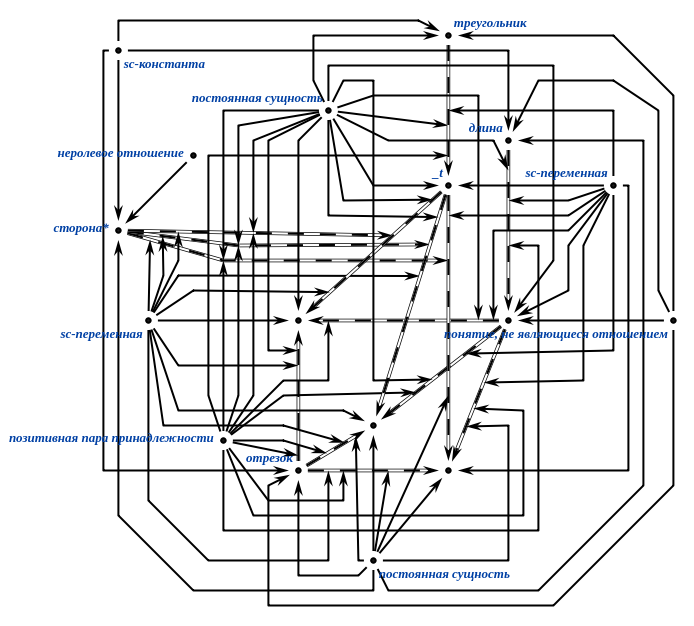
\includegraphics[scale=0.5]{./figures/intro/scg/examples/scg_examples_transf_1_1.png}
\end{frame}

\begin{frame}{\\SCg-code: Transformation examples (1)}
\topline
\justifying
\vspace*{\fill}\\
\vspace{10mm}
\centering
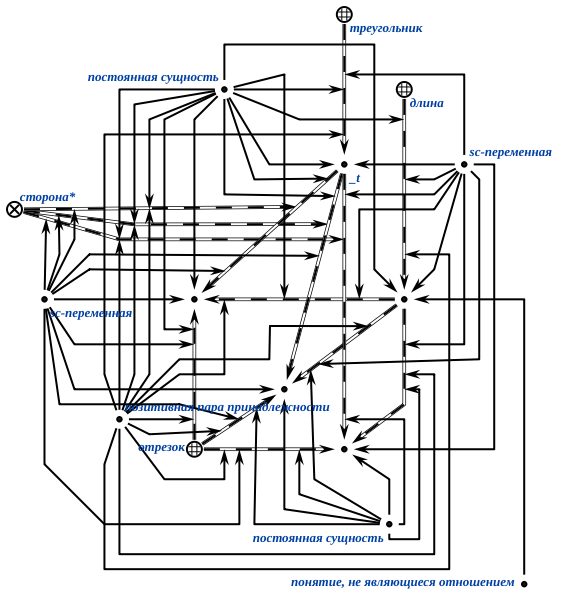
\includegraphics[scale=0.5]{./figures/intro/scg/examples/scg_examples_transf_1_2.png}
\end{frame}

\begin{frame}{\\SCg-code: Transformation examples (1)}
\topline
\justifying
\vspace*{\fill}\\
\vspace{10mm}
\centering
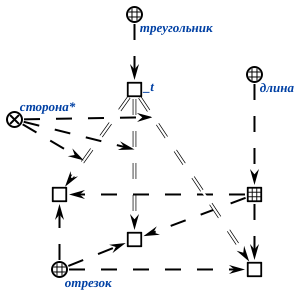
\includegraphics[scale=0.5]{./figures/intro/scg/examples/scg_examples_transf_1_3.png}
\end{frame}

\begin{frame}{\\SCg-code: Transformation examples (1)}
\topline
\justifying
\vspace*{\fill}\\
\vspace{10mm}
\centering
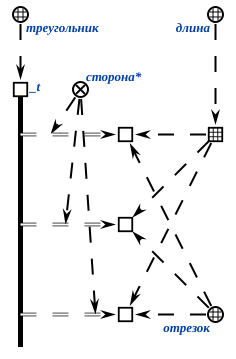
\includegraphics[scale=0.5]{./figures/intro/scg/examples/scg_examples_transf_1_4.png}
\end{frame}

\begin{frame}{\\SCg-code: Transformation examples (2)}
\topline
\justifying
\vspace*{\fill}\\
\vspace{10mm}
\centering
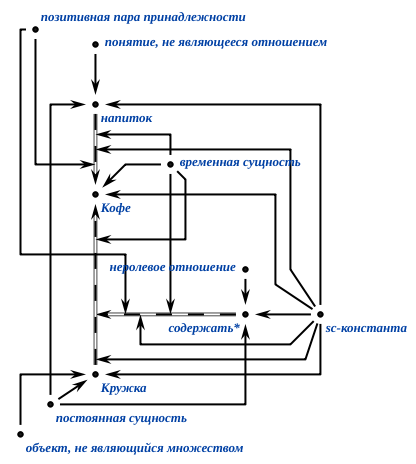
\includegraphics[scale=0.5]{./figures/intro/scg/examples/scg_examples_transf_2_1.png}
\end{frame}

\begin{frame}{\\SCg-code: Transformation examples (2)}
\topline
\justifying
\vspace*{\fill}\\
\vspace{10mm}
\centering
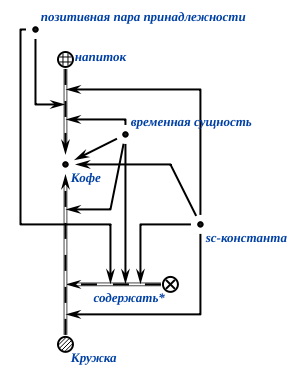
\includegraphics[scale=0.5]{./figures/intro/scg/examples/scg_examples_transf_2_2.png}
\end{frame}

\begin{frame}{\\SCg-code: Transformation examples (2)}
\topline
\justifying
\vspace*{\fill}\\
\vspace{10mm}
\centering
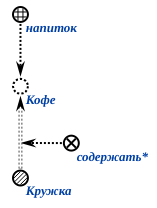
\includegraphics[scale=0.5]{./figures/intro/scg/examples/scg_examples_transf_2_3.png}
\end{frame}

\begin{frame}{\\SCg-code: Transformation examples (3)}
\topline
\justifying
\vspace*{\fill}\\
\vspace{10mm}
\centering
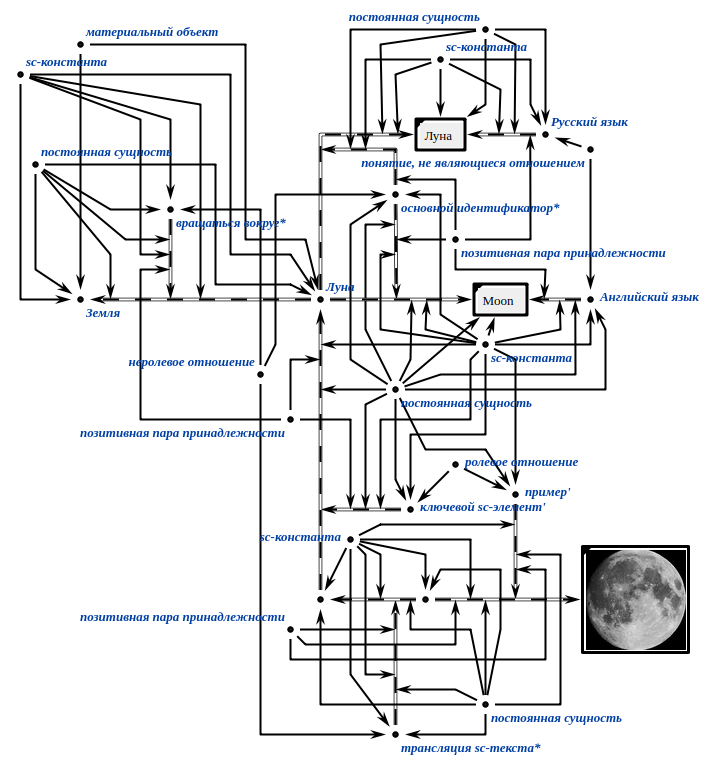
\includegraphics[scale=0.4]{./figures/intro/scg/examples/scg_examples_transf_3_1.png}
\end{frame}

\begin{frame}{\\SCg-code: Transformation examples (3)}
\topline
\justifying
\vspace*{\fill}\\
\vspace{10mm}
\centering
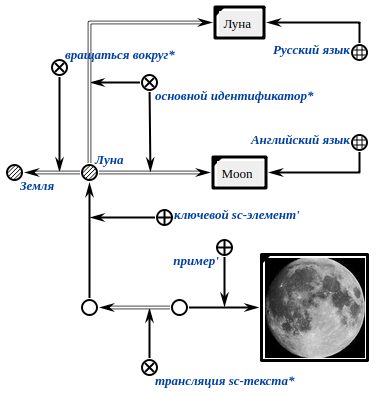
\includegraphics[scale=0.5]{./figures/intro/scg/examples/scg_examples_transf_3_2.png}
\end{frame}

\begin{frame}{\\SCg-code: Transformation examples (3)}
\topline
\justifying
\vspace*{\fill}\\
\vspace{10mm}
\centering
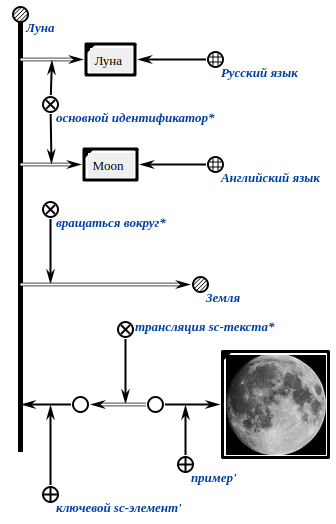
\includegraphics[scale=0.5]{./figures/intro/scg/examples/scg_examples_transf_3_3.png}
\end{frame}

\begin{frame}
\centering
\Huge
SCs-code
\end{frame}

\begin{frame}{\\SCs-code}
\topline
\justifying
\vspace*{\fill}\\
\begin{SCn}
	\scnheader{SCs-code}
	\scnidtf{Semantic Code string}
	\scnidtf{Linear knowledge representation language for ostis-systems}
	\scnidtf{variety of SCs-code texts}
	\scnidtf{Language of external linear representation of constructions of the internal language of ostis-systems}
	\scntext{\textit{explanation}}{SCs-code is a set of linear texts \textit{(sc.s-texts)}, each of which consists of sentences \textit{(sc.s-sentences)}, separated from each other by \textit{double semicolons} (the \textit{sc.s-sentence separator}). A \textit{sc.s-sentence} is a sequence of \textit{sc-identifiers}, which are the names of the entities being described and separated from each other by various \textit{sc.s-separators} and \textit{sc.s-delimiters}.}
\end{SCn}
\end{frame}

\begin{frame}{\\SCs-code syntax}
\topline
\justifying
\vspace*{\fill}\\
\small{
	\begin{SCn}
		\scnheader{SCs-code Alphabet}
		\scnidtf{SCs-code character alphabet}
		\scnidtf{set of SCs-code characters}
		\scnidtf{symbol used in SCs-code texts}
		\scnidtf{Language of external linear representation of constructions of the internal language of ostis-systems}
		\scntext{\textit{explanation}}{\textit{SCs-code alphabet} is built on the basis of modern generally accepted character sets, which allows for simplifying the development of tools for working with \textit{sc.s-texts} using modern technologies.
			
			\textit{sc.s-texts}, like texts of any other language that are variants of the external display of SC-code texts, may contain various files, including natural language files or even files containing other \textit{sc.s-texts}. In general, such files may use a wide variety of characters, so we will assume that these characters are not included in the \textit{SCs-code alphabet}.
		\end{SCn}
	}
\end{frame}

\begin{frame}{\\SCs-code syntax}
	\topline
	\justifying
	\vspace*{\fill}\\
	\vspace{10mm}
	To simplify the process of developing source texts of knowledge bases using SCs-code and creating corresponding tools, two alphabets of symbols are introduced:
	\begin{textitemize}
		The \item \textbf{Basic Alphabet} of characters used in \textit{sc.s-connectors} includes only characters included in the portable character set and found on a standard modern keyboard. Therefore, a standard text editor is sufficient for developing knowledge base source texts that use only the \textit{Basic Alphabet} of characters used in \textit{sc.s-connectors}.
		The extended alphabet of symbols used in sc.s connectors also includes additional symbols that make sc.s texts (and sc.n texts) more readable and visual. Visualizing and developing sc.s texts using the extended alphabet requires specialized tools.
	\end{textitemize}
\end{frame}

\begin{frame}{\\SCs-code syntax}
	\topline
	\justifying
	\vspace*{\fill}\\
	\vspace{10mm}
	Both the \textit{Basic} and \textit{Extended sc.s-connector Alphabets} use the following general features to characterize the type of \textit{sc-connector} being represented:
	\begin{textitemize}
		\item underscore as a sign of variable images \\ \textit{sc-connectors} (one underscore for \textit{sc-connectors} that are primary \textit{sc-variables}, two underscores for \textit{sc-connectors} that are secondary \textit{sc-variables (sc-metavariables))};
		\item vertical bar “ | ” as a feature of images \textit{negative sc-arcs of belonging};
		\item slash “ / ” as a feature of images \textit{fuzzy sc-arcs of membership};
		\item tilde “ $\sim$ ” as a feature of images of \textit{temporal sc-arcs of membership}.
	\end{textitemize}
\end{frame}

\begin{frame}{\\SCs-code syntax}
	\topline
	\justifying
	\vspace*{\fill}\\
	\small
	\begin{SCn}
		\scnheader{Alphabet of characters used in sc.s separators}
		\scnhaselement{\textit{space}; \textit{semicolon}; \textit{colon}; \textit{circle bullet}; \textit{equal sign}}
		\scnsuperset{Alphabet of characters used in sc.s-separators depicting incidence relationships of sc-elements}
		\begin{scnindent}
			\scnhaselement{![ > ]!; ![ < ]!; ![ | ]!; ![ - ]!;}
		\end{scnindent}
		\scnsuperset{Alphabet of characters used in sc.s connectors}
		\begin{scnindent}
			\scnsuperset{Extended alphabet of symbols used in sc.s connectors}
			\begin{scnindent}
				\scnidtf{Extended sc.s Connector Alphabet}
				\scnhaselement{![$\in$]!; ![$\ni$]!; ![$\notin$]!; ![$\not\ni$]!; ![$\subseteq$]!; ![$\supseteq$]!; ![$\subset$]!; ![$\supset$]!; ![$\leq$]!; ![$\geq$]!; ![$\Leftarrow$]!; ![$\Rightarrow$]!; ![$\Leftrightarrow$]!; ![$\leftarrow$]!; ![$\rightarrow$]!; ![$\leftrightarrow$]!}
			\end{scnindent}
			\scnsuperset{Base alphabet of symbols used in sc.s connectors}
			\begin{scnindent}
				\scnidtf{Basic alphabet of sc.s-connectors}
				\scnhaselement{![$\sim$]!; ~\textit{underscore}; ~\textit{equal sign}; ![ > ]!; ~![<]!; ~\textit{colon}; ![ - ]!; ![ | ]!; ![ / ]!;}
			\end{scnindent}
		\end{scnindent}
	\end{SCn}
\end{frame}

\begin{frame}{\\SCs-code syntax}
	\topline
	\justifying
	\vspace*{\fill}\\
	\begin{SCn}
		\scnheader{Alphabet of characters used in sc.s delimiters}
		\scnhaselement{![ ( ]!; ![ ) ]!; ![ * ]!;}
		
		\scnheader{Alphabet of symbols used in ambiguous sc.s images of sc-nodes}
		\scnhaselement{![ \{ ]!; ![ \} ]!; ![ ! ]!; ![ - ]!; ![ [ ]!; ![ ] ]!;}
	\end{SCn}
\end{frame}

\begin{frame}{\\Denotational semantics of SCs-code}
	\topline
	\justifying
	\vspace*{\fill}\\
	\begin{SCn}
		\begin{figure}[H]
			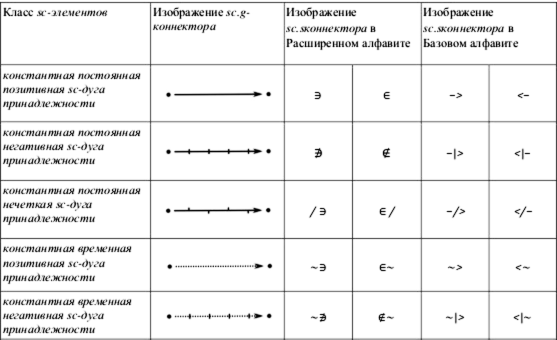
\includegraphics[scale=0.5]{./figures/external_langs/table_scs_1.png}
		\end{figure}
	\end{SCn}
\end{frame}

\begin{frame}{\\Denotational semantics of SCs-code}
	\topline
	\justifying
	\vspace*{\fill}\\
	\begin{SCn}
		\begin{figure}[H]
			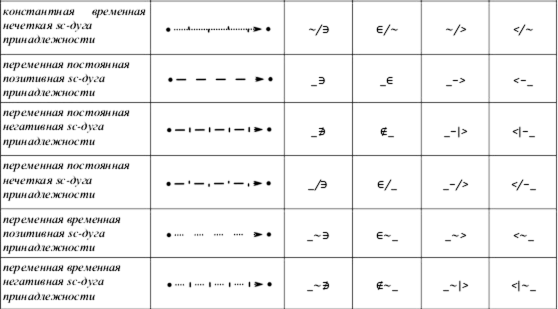
\includegraphics[scale=0.5]{./figures/external_langs/table_scs_2.png}
		\end{figure}
	\end{SCn}
\end{frame}

\begin{frame}{\\Denotational semantics of SCs-code}
	\topline
	\justifying
	\vspace*{\fill}\\
	\begin{SCn}
		\begin{figure}[H]
			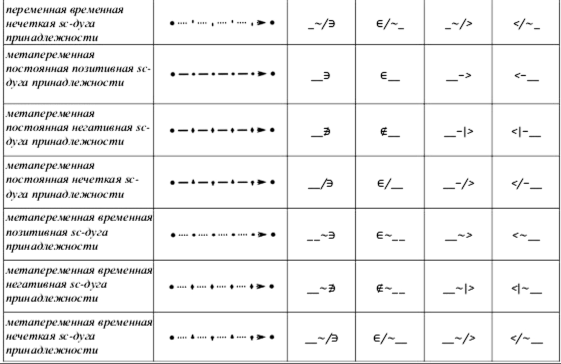
\includegraphics[scale=0.5]{./figures/external_langs/table_scs_3.png}
		\end{figure}
	\end{SCn}
\end{frame}

\begin{frame}{\\SCs-code: Transformation examples}
	\topline
	\justifying
	\vspace*{\fill}\\
	\vspace{10mm}
	\scriptsize
	
	\begin{SCn}
		\scnfilelong{\textit{inclusion* $\ni$ pair1;;\\inclusion* $\ni$ pair2;;\\inclusion* $\ni$ pair3;;\\inclusion* $\ni$ pair4;;\\inclusion* $\ni$ pair5;;\\side* $\ni$ pair1;;\\side* $\ni$ pair2;;\\side* $\ni$ pair3;;\\side* $\ni$ pair4;;\\side* $\ni$ pair5;;\\Quad(DtA;DtB;DtC;DtD) |- pair1 >| Neg(DtB;DtC);;\\Quad(DtA;DtB;DtC;DtD) |- pair2 >| Neg(PointC,PointD);;\\Treugk(PointB,PointC,PointD) |- pair3 >| Neg(PointV,PointS);;\\Treugk(PointV,PointS,PointD) |- pair4 >| Neg(PointC,PointD);;\\Treugk(PointB,PointC,PointD) |- pair5 >| Neg(PointB;PointD);;\\quadrilateral $\ni$ Quadrilateral(PointA;PointB;PointC;PointD);;\\triangle $\ni$ Triangle(PointB;PointC;PointD);;\\link1 |- pair6 >| Treugk(PointV;PointC;PointD);;\\figure decomposition* $\ni$ pair6;;\\link1 $\ni$ Neg(PointV;PointC);;\\link1 $\ni$ Neg(PointC;PointD);;\\link1 $\ni$ Neg(PointV;PointD);;}}
	\end{SCn}
	
\end{frame}

\begin{frame}{\\SCs-code: Transformation examples}
	\topline
	\justifying
	\vspace*{\fill}\\
	\vspace{10mm}
	
	\begin{figure}[H]
		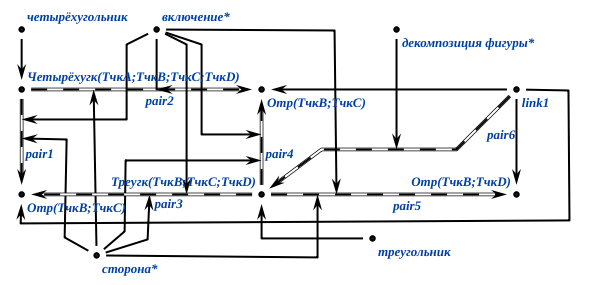
\includegraphics[scale=0.5]{./figures/intro/scs/scs_transf_example.png}
	\end{figure}
	
\end{frame}

\begin{frame}{\\SCs-code: Transformation examples}
	\topline
	\justifying
	\vspace*{\fill}\\
	\vspace{10mm}
	\scriptsize
	
	\begin{SCn}
		\scnfilelong{\textit{side* $\ni$ (Four-arm(PointA,PointB,PointC,PointD) $\Rightarrow$ Neg(PointB,PointC));;\\side* $\ni$ (Four-point(PointA,PointV,PointC,PointD) $\supseteq$ Neg(PointC;PointD));;\\side* $\ni$ (Treugk(PointV;PointC;PointD) $\supseteq$ Neg(PointV;PointC));;\\side* $\ni$ (Treugk(PointV;PointC;PointD) $\supseteq$ Neg(PointC;PointD));;\\side* $\ni$ (Treugk(PointB,PointC,PointD) $\supseteq$ Neg(PointB,PointD));;\\Fourfold(PointA,PointB,PointC,PointD) $\supseteq$ Neg(PointA;PointC); Neg(PointV;PointS);;\\Treugk(PointV;PointC;PointD) $\supseteq$ Neg(PointC;PointD); Treugk(PointV,PointC,PointD); Neg(PointV,PointD);;}}
	\end{SCn}
	
\end{frame}

\begin{frame}{\\SCs-code: Transformation examples}
	\topline
	\justifying
	\vspace*{\fill}\\
	\vspace{10mm}
	\scriptsize
	
	\begin{SCn}
		\scnfilelong{\textit{Four-arc(PointA,PointB,PointC,PointD) $\supseteq$ side*: Neg(PointA,PointC);\\Four-arc(PointA,PointV,PointC,PointD) $\supseteq$ side*: Neg(PointC;PointD); Neg(PointC,PointD);;\\Treugk(PointB,PointC,PointD) $\supseteq$ side*: Neg(PointB;PointD);;\\quadrilateral $\ni$ Quadrilateral(PointA;PointB;PointC;PointD);;\\triangle $\ni$ Triangle(PointB;PointC;PointD);;\\link1 $\Rightarrow$decomposition of the figure*: Treugk(PointV;PointC;PointD);;\\link1 $\ni$ Neg(PointV;PointC);;\\link1 $\ni$ Neg(PointC;PointD);;\\link1 $\ni$ Neg(PointV;PointD);;}}
	\end{SCn}
	
\end{frame}

\begin{frame}{\\SCs-code: Transformation examples}
	\topline
	\justifying
	\vspace*{\fill}\\
	\vspace{10mm}
	\scriptsize
	
	\begin{SCn}
		\scnfilelong{\textit{Four (PointA,PointB,PointC,PointD) $\supseteq$ side*: Neg(PointB,PointC); Neg(PointC;PointD); Ref(PointC;PointD); Neg(PointB,PointD); Treugk(PointV;PointS;PointD);;\\link1 $\ni$ Neg(PointV;PointS); Ref(PointC;PointD); Neg(PointV,PointD);;}}
	\end{SCn}
	
\end{frame}

\begin{frame}{\\SCs-code: Transformation examples}
	\topline
	\justifying
	\vspace*{\fill}\\
	\vspace{10mm}
	\scriptsize
	
	\begin{SCn}
		\scnfilelong{\textit{quadrilateral $\ni$ Quadrangle(PointA;PointB;PointC;PointD)\\ (* $\supseteq$ side*: Neg(PointB;PointC); Neg(PointC;PointD);; *);;\\triangle $\ni$ Triangle(PointB;PointC;PointD) \\(* $\supseteq$ side*: Neg(PointB;PointC); Neg(PointC;PointD); Neg(PointB;PointD);; *);;\\Treugk(PointB;PointC;PointD) $\Leftarrow$decomposition of figure*: link1 (* $\ni$ Neg(PointB;PointC); Ref(PointC;PointD); Otr(TchkV;TchkD);; *);;}}
	\end{SCn}
	
\end{frame}

\begin{frame}
	\centering
	\Huge
	SCn-code
\end{frame}

\begin{frame}{\\SCn-code}
	\topline
	\justifying
	\vspace*{\fill}\\
	\small{
		\begin{SCn}
			\scnheader{SCn-code}
			\scnidtf{Semantic Code natural}
			{Ostis-systems structured knowledge representation language}
			\scnidtf{Language of external formatted representation of constructions of the internal language of ostis-systems}
			
			\scntext{explanation}{\textit{SCn-code} is a language for the structured external representation of \textit{SC-code} texts and is a syntactic extension of \textit{SCs-code}, aimed at increasing the clarity and compactness of \textit{SCs-code} texts.
				
				\textit{SCn-code} enables the transition from linear \textit{SCs-code} texts to formatted and effectively two-dimensional texts, in which the original linear \textit{SCs-code} text is decomposed into lines arranged "vertically". The beginning of all text lines is fixed and determined by a known and limited set of rules, making it possible to use this when formatting \textit{sc.n-text}.
			\end{SCn}
		}
	\end{frame}
	
	\begin{frame}{\\SCn-code}
		\topline
		\justifying
		\vspace*{\fill}\\
		An important feature of the \textit{SCn-code} is the "two-dimensional"{} nature of its texts. This is manifested in the fact that for each fragment of the \textit{SCn-code} text, the amount of indentation from the left is of great importance
		edges of the line.
		
		In the text of the \textit{SCn-code}, unlike the text of the \textit{SCs-code}, for each fragment of text it is important not only how this fragment is related to other fragments "horizontally"{} (which fragment is \underline{to the left} and which is \underline{to the right} on the same \textit{line}), but also how it is related to other fragments "vertically"{} (which fragment is \underline{above} on the previous line and which is \underline{below} on the next line).
		
		So, for example, if in the text of the \textit{SCn-code} some \textit{sc-identifier} (external identifier of the \textit{sc-element}) is placed immediately after the vertical tabulation line and some \textit{sc.s-connector} is placed exactly below it, this means that the specified \textit{sc-element} is incident to the \textit{sc-connector} depicted by the specified \textit{sc.s-connector}.
	\end{frame}
	
	\begin{frame}{\\SCn-code syntax}
		\topline
		\justifying
		\vspace*{\fill}\\
		The alphabet of symbols of the \textit{SCs-code} is also the alphabet of symbols of the \textit{SCn-code}, i.e. the \textit{alphabets*} of these languages coincide.
		\textit{SCn-code} -- a language, each \textit{text} of which is specified:
		\begin{textitemize}
			\item by the set of \textit{symbols} included in it;
			\item relation of the order (sequence) of \textit{symbols} along the "horizontal";
			\item relation of the order (sequence) of \textit{symbols} along the "vertical"{}.
		\end{textitemize}
	\end{frame}
	
	\begin{frame}{\\SCn-code syntax}
		\topline
		\justifying
		\small{
			\begin{SCn}
				\scnheader{sc.n-text}
				\scnidtf{SCn-code text}
				\scnidtf{SCn-code sentence sequence}
				\scnidtf{sequence of SCn-code sentences, each of which is not part of any other sentence from \underline{this} sequence}
				
				\scnheader{scn-text page}
				\scnidtf{page where sc.n-text is located}
				
				\scnheader{scn-text markup line}
				\scnidtf{sc.n-text tabulation line}
				\scnidtf{vertical line marking sc.n text}
				\scnidtf{vertical line used to simplify the perception of sc.n-texts and indicating the indentation level for components of sc.n-sentences}
			\end{SCn}
		}
	\end{frame}
	
	\begin{frame}{\\SCn-code syntax}
		\topline
		\justifying
		\vspace*{\fill}\\
		\small{
			All components of \textit{sc.s-texts} are also used in \textit{sc.n-texts}:
			\begin{textitemize}
				\item \textit{sc-identifiers, sc.s-connectors}, \textit{sc.s-connectors} modifiers with corresponding separators (colons);
				\item separators used in \textit{sc-expressions} denoting \textit{sc-sets} specified by listing elements with appropriate separators (semicolon or circle marker);
				\item round markers in enumerations of \textit{sc-elements} identifiers, connected by the same type of \textit{sc-connectors} with the same type of modifiers with a given \textit{sc-element};
				\item sentence separators (double semicolons) (omitted when converting \textit{sc.s-sentences} to \textit{sc.n-sentences});
				\item delimiters of attached \textit{sc.s-sentences} (omitted when converting \textit{sc.s-sentences} to \textit{sc.n-sentences}).
			\end{textitemize}
		}
	\end{frame}
	
	\begin{frame}{\\SCn-code syntax}
		\topline
		\justifying
		\vspace*{\fill}\\
		Unlike \textit{sc.s-texts}, in \textit{sc.n-texts}:
		\begin{textitemize}
			\item new types of \textit{sc-expressions} are added (namely, \textit{sc-expressions} that have a two-dimensional character);
			\item a new type of sentence separator is added - an empty line;
			\item the placement of sentences is changed taking into account the two-dimensional nature of such placement.
		\end{textitemize}
	\end{frame}
	
	\begin{frame}{\\Denotational semantics of the SCn-code}
		\topline
		\justifying
		\vspace*{\fill}\\
		Unlike \textit{sc.s-texts}: in \textit{sc.n-texts, an sc.s-connector} can be incident with the preceding \textit{sc-identifier} (both a simple one and a \textit{sc-expression}) not only "horizontally"{}, but also "vertically"{}. For this, the \textit{sc.s-connector} is placed strictly \underline{under} the preceding \textit{sc-identifier}.\\ Moreover, "vertically"{}, a \textit{sc-identifier} can be incident not with one, but \underline{several} \textit{sc.s-connectors}, which are successively "vertically"{} placed under the specified \textit{sc-identifier}. This allows, within the framework of one \textit{sc.n-sentence}, to represent an arbitrary number of "branches"{} from each \textit{sc-identifier}, i.e. an arbitrary number of \textit{sc.s-connectors}, incident to this \textit{sc-identifier}.
		
		Each \textit{sc-identifier}, including a \textit{sc-expression}, must be placed immediately to the right of the vertical guideline if a \textit{sc.s-connector} is placed \underline{below it}.
	\end{frame}
	
	\begin{frame}{SCn-code: Operation of transforming an sc.s-sentence into an sc.n-sentence}
		\topline
		\justifying
		\vspace*{\fill}\\
		\begin{SCn}
			\scnfilelong{\textit{Treugk(PointV;PointS;PointD)} $\Rightarrow$ \textit{side*}: \textit{Opt(PointV;PointS)} (* $\in$ \textit{segment};; *);;}
			
			\noindent\rule{12cm}{1.5pt}		
			
			\scnheader{Treugk(PointV,PointC,PointD)}
			\scnrelfrom{side}{Otr(TchkV;TchkS)}
			\begin{scnindent}
				\scniselement{segment}
			\end{scnindent}
			
		\end{SCn}
	\end{frame}
	
	\begin{frame}{SCn-code: Operation of joining an sc.n-sentence}
		\topline
		\justifying
		\vspace*{\fill}\\
		\begin{SCn}
			\scnheader{Treugk(PointV,PointC,PointD)}
			\scnrelfrom{side}{Otr(TchkV;TchkS)}
			
			\scnheader{Отр(ПчкВ;ПчкС)}
			\scniselement{segment}
			
			\noindent\rule{12cm}{1.5pt}
			
			\scnheader{Treugk(PointV,PointC,PointD)}
			\scnrelfrom{side}{Otr(TchkV;TchkS)}
			\begin{scnindent}
				\scniselement{segment}
			\end{scnindent}
			
		\end{SCn}
	\end{frame}
	
\fi